% Created 2021-09-11 Sat 08:17
% Intended LaTeX compiler: xelatex
\documentclass[letterpaper]{article}
\usepackage{graphicx}
\usepackage{grffile}
\usepackage{longtable}
\usepackage{wrapfig}
\usepackage{rotating}
\usepackage[normalem]{ulem}
\usepackage{amsmath}
\usepackage{textcomp}
\usepackage{amssymb}
\usepackage{capt-of}
\usepackage{hyperref}
\usepackage[margin=1in]{geometry}
\usepackage{fontspec}
\usepackage{indentfirst}
\setmainfont[ItalicFont = LiberationSans-Italic, BoldFont = LiberationSans-Bold, BoldItalicFont = LiberationSans-BoldItalic]{LiberationSans}
\newfontfamily\NHLight[ItalicFont = LiberationSansNarrow-Italic, BoldFont       = LiberationSansNarrow-Bold, BoldItalicFont = LiberationSansNarrow-BoldItalic]{LiberationSansNarrow}
\newcommand\textrmlf[1]{{\NHLight#1}}
\newcommand\textitlf[1]{{\NHLight\itshape#1}}
\let\textbflf\textrm
\newcommand\textulf[1]{{\NHLight\bfseries#1}}
\newcommand\textuitlf[1]{{\NHLight\bfseries\itshape#1}}
\usepackage{fancyhdr}
\pagestyle{fancy}
\usepackage{titlesec}
\usepackage{titling}
\makeatletter
\lhead{\textbf{\@title}}
\makeatother
\rhead{\textrmlf{Compiled} \today}
\lfoot{\theauthor\ \textbullet \ \textbf{2021-2022}}
\cfoot{}
\rfoot{\textrmlf{Page} \thepage}
\titleformat{\section} {\Large} {\textrmlf{\thesection} {|}} {0.3em} {\textbf}
\titleformat{\subsection} {\large} {\textrmlf{\thesubsection} {|}} {0.2em} {\textbf}
\titleformat{\subsubsection} {\large} {\textrmlf{\thesubsubsection} {|}} {0.1em} {\textbf}
\setlength{\parskip}{0.45em}
\renewcommand\maketitle{}
\author{Houjun Liu}
\date{\today}
\title{Water with Paul}
\hypersetup{
 pdfauthor={Houjun Liu},
 pdftitle={Water with Paul},
 pdfkeywords={},
 pdfsubject={},
 pdfcreator={Emacs 27.2 (Org mode 9.4.4)}, 
 pdflang={English}}
\begin{document}

\maketitle


\section{Alright, let's talk about water.}
\label{sec:org004d9ab}
\begin{figure}[htbp]
\centering
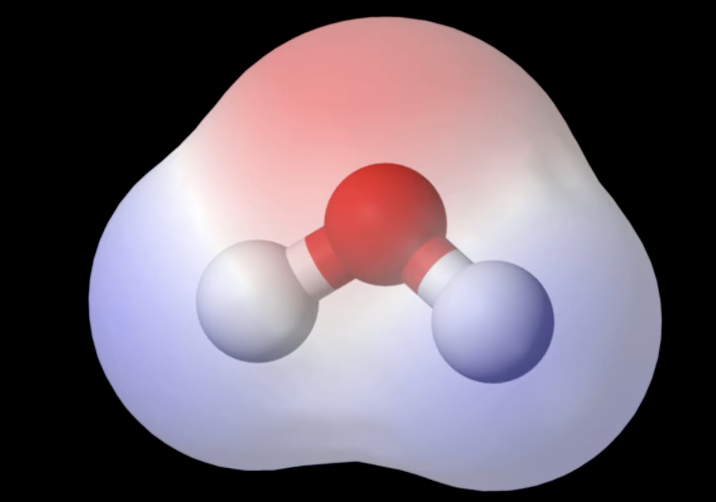
\includegraphics[width=.9\linewidth]{./Screen Shot 2020-08-24 at 10.08.34 PM.png}
\caption{Watah!}
\end{figure}

\subsection{Intra-Molecular water bonds}
\label{sec:orgb841aed}
\begin{itemize}
\item As we know (or looked up from the PTable)
\item Hydrogen has electronegativity of 2.20, and oxygen has EN 3.44
\item The difference >0.4 <1.7 makes these bonds \textbf{polar covalent}
\end{itemize}

See \href{KBhBIO101BondingReview.org}{KBhBIO101BondingReview}, bonding
review

\href{Test.org}{Test}

\subsection{Why is ice less dense?}
\label{sec:org486bdd1}
\begin{itemize}
\item Freezing usually bring new ordering of molecules to make it paced
\item But! Not the case for normal water because of hydrogen bond

\begin{itemize}
\item Strong 6-ring Hydrogen bonds in ice prevents shrinking
\item Empty space filled with air, making it less dense
\end{itemize}
\end{itemize}

\subsubsection{Why do I care?}
\label{sec:orgbfc4300}
Ice floats! Causing beautiful ice effects that the ecosystem uses

\begin{itemize}
\item Pseudo-landmass

\begin{itemize}
\item Antarctica
\item Animal habitat
\end{itemize}

\item Ice reflect incoming light ("albeto")

\begin{itemize}
\item Bounces energy off
\item Cools the water
\end{itemize}
\end{itemize}

\subsection{Inter-Molecular water bonds properties}
\label{sec:org9ea19b7}
See \href{KBhBIO101PropsOfWater.org}{KBhBIO101PropsOfWater},
properties of water.

\section{So, why is water the chosen liquid?}
\label{sec:orgffd7d51}
See also \href{KBhBIO101PropsOfWater.org}{KBhBIO101PropsOfWater}
Properties of Water

\begin{itemize}
\item Liquid at Earth temperatures
\item Sticky => strong bonds that help water hold together + resist change
in temperature (hence why AlcaholLand cannot exist).

\begin{itemize}
\item Varing te (incomplete \#todo-houjun @jemoka)
\end{itemize}

\item Is universal solvent
\end{itemize}
\end{document}
